\documentclass[9pt,a4paper]{extarticle}


	\usepackage[margin=5em,bottom=8em]{geometry}


%1 est la marge gauche
%2 est la marge en haut
%3 est la marge droite
%4 est la marge en bas
%5 fixe la hauteur de l'entête
%6 fixe la distance entre l'entête et le texte
%7 fixe la hauteur du pied de page
%8 fixe la distance entre le texte et le pied de page
%------------------------------Packages généraux------------------------------

\usepackage[english]{babel}
\usepackage[T1]{fontenc}
\usepackage{ae}
\usepackage[utf8]{inputenc}
\usepackage{scrextend}
\usepackage{hyperref}
 \hypersetup{
    colorlinks = true,
    linkcolor=black,
    urlcolor = black
    }
%-------------------------Mathématiques------------------------------
\usepackage{amsmath}
\usepackage{amssymb}
\usepackage{amsthm}
\usepackage{amsfonts}
\usepackage{eucal}
\newcommand\independent{\protect\mathpalette{\protect\independenT}{\perp}}
\def\independenT#1#2{\mathrel{\rlap{$#1#2$}\mkern2mu{#1#2}}}
%-----------------------Codes et algorithmes--------------------------
\usepackage{algorithm}
%\usepackage{algorithmic}
%\usepackage{clrscode3e}
\usepackage[noend]{algpseudocode}
%\newcommand{\pushline}{\Indp}% Indent
%\newcommand{\popline}{\Indm\dosemic}% Undent
%\newcommand{\nonl}{\renewcommand{\nl}{\let\nl\oldnl}}%


%------------------------------Graphics------------------------------

\usepackage{graphicx}
\usepackage{fancyhdr}
\usepackage{fancybox}
\usepackage{color}
\usepackage{pgf, tikz}
\usetikzlibrary{arrows, automata}
%\usepackage{slashbox}

%------------------Sub-sections--------%
\usepackage{titlesec}
\usepackage{hyperref}
\usepackage{comment}

\usepackage{hyperref}
               
 \hypersetup{
    colorlinks = true,
    linkcolor=black,
    urlcolor = black
    }
    
\newenvironment{solution}
    {%\begin{center}
    %\begin{tabular}{|p{0.9\textwidth}|}
    %\hline\\
    \color{red}
    }
    { 
    %\\\\\hline
    %\end{tabular} 
    %\end{center}
    \color{black}
    }
    
\newcommand{\blue}[1]{\textcolor{blue}{#1}}


\newif\ifhideproofs
%\hideproofstrue %uncomment to hide proofs

\ifhideproofs
\usepackage{environ}
\NewEnviron{hide}{}
\let\solution\hide
\let\endsolution\endhide
\fi

\title{{\bf INFO8006 Introduction to Artificial Intelligence}\\[1em]
Exercises 1: Solving problems by searching}
\date{}
%------------------------------Début du document------------------------------
\begin{document}
\maketitle
\vspace{-4em}
%------------------------------Page de garde------------------------------

  \section*{Learning outcomes}
  At the end of this exercise session you should be able to:
\begin{itemize}
   \item formulate search problems rigorously.
   \item theoretically analyse the algorithms to perform uninformed search (depth-first, breadth-first, uniform-cost) and informed search (greedy-search, $\text{A}^\star$).
   \item apply each of these algorithms on search problems defined in fully observable and deterministic environments.
\end{itemize}

   \section*{Exercise 1: Search algorithms}
   \begin{center}
       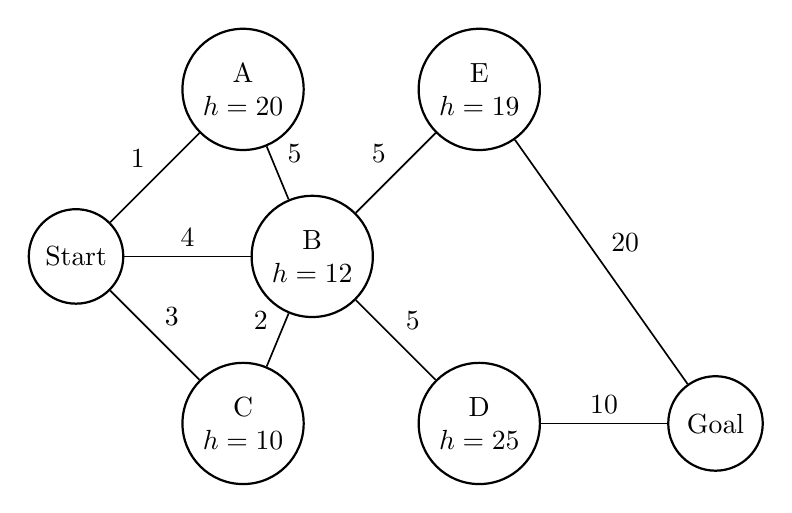
\begin{tikzpicture}[
            -> = stealth, % arrow head style
            %shorten > = 1pt, % don't touch arrow head to node
            auto,
            node distance = 3cm, % distance between nodes
            semithick % line style
        ]

        \tikzstyle{every state}=[
            draw = black,
            thick,
            fill = white,
            minimum size = 12mm
        ]

        \node[state, align=center] (S) {Start};
        \node[state, align=center] (A) [above right of=S] {A\\$h=20$};
        \node[state, align=center] (B) [right of=S] {B\\$h=12$};
        \node[state, align=center] (C) [below right of=S] {C\\$h=10$};
        \node[state, align=center] (D) [below right of=B] {D\\$h=25$};
        \node[state, align=center] (E) [above right of=B] {E\\$h=19$};
        \node[state, align=center] (F) [right of=D] {Goal};

        \path[-] (S) edge node {1} (A);
        \path[-] (S) edge node {4} (B);
        \path[-] (S) edge node {3} (C);
        \path[-] (B) edge node {5} (D);
        \path[-] (B) edge node {5} (E);
        \path[-] (D) edge node {10} (F);
        \path[-] (E) edge node {20} (F);
        \path[-] (C) edge node {2} (B);
        \path[-] (A) edge node {5} (B);

        %\draw[red, dashed] (1, 2) -- (1, -2);
    \end{tikzpicture}
   \end{center}
    For each of the following search algorithms, give the order in which states are expanded as well as the final path returned by the algorithm. If two nodes are in competition to be expanded, the conflict is resolved by alphabetical order.
    \begin{solution}
    \\
    Here follows a search algorithm which is valid for non-consistent (but admissible) heuristics.
\begin{algorithm}[H]
\caption{Graph-Search Algorithm}\label{algo:GS}
\begin{tabular}{ll}
    \textit{Input:}  & $\text{fringe}$: The fringe, which is a priority queue for nodes, \textbf{initialised with the starting node}. \\
     & $\text{closed}$: A list of closed nodes, \textbf{initially empty}.\\
     \textit{Output:}  & $p$: A list of nodes which represents the optimal path.\\
\end{tabular}
\small
\begin{algorithmic}[1]
\Procedure{Graph-Search}{$\text{fringe}, \text{closed}$}
\While{$True$}
\State $n \gets \text{fringe}.pop()$ %\Comment{Pop the node with highest priority}
\If{$n \text{ is } nil$}
 \State \Return $nil$
\EndIf
\If{$n.isGoal()$}
   \State \Return $n.getPath()$
\EndIf
\State $\text{closed}.append(n)$
\For{$n' \in n.children$}
    \State $p \gets n'.computePriority(n)$
    \If{$n' \not\in \text{closed} \quad \&\& \quad n' \not\in \text{fringe}$}
    \State $n'.setPriority(p)$
    \State $n'.setParent(n)$
    \State $\text{fringe}.push(n')$
    
    \ElsIf{$n' \in \text{fringe} \quad \&\& \quad p < \text{fringe}.get(n').getPriority()$}
    \State $\text{fringe}.remove(n')$
    \State $\text{fringe}.push(n')$
    
    \ElsIf{$n' \in \text{closed} \quad \&\& \quad p < \text{closed}.get(n').getPriority()$}
    \State $\text{closed}.remove(n')$
    \State $\text{fringe}.push(n')$
    \EndIf
\EndFor
\EndWhile
\EndProcedure
\end{algorithmic}
\vspace{1em}
\end{algorithm}
    \end{solution}

    \begin{enumerate}
        \item Depth-First search
        %\begin{comment}
        %coccu
        %\end{comment}
        \begin{solution}
        \\
        Expansion: S, A, B, D, Goal \\
        Path: S $\rightarrow$ A $\rightarrow$ B $\rightarrow$ D $\rightarrow$ G \\
        We use a LIFO heap to perform the search. In order to prevent cycles, when we add a node into the heap we replace its previous version if there is one and we never add a node that has already been expanded.\\
        Step-by-step:
        \begin{itemize}
            \item Heap = \{S()\}; Expand(S); Visited = \{S()\}
            \item Heap = \{A(S), B(S), C(S)\}; Expand(A(S)); Visited = \{S(), A(S)\}
            \item Heap = \{B(A), C(S)\}; Expand(B(A)); Visited = \{S(), A(S), B(A)\}
            \item Heap = \{C(B), D(B), E(B)\}; Expand(C(B));  Visited = \{S(), A(S), B(A), C(B)\}
            \item Heap = \{D(B), E(B)\}; Expand(D(B)); Visited = \{S(), A(S), B(A), C(B), D(B)\}
            \item Heap = \{Goal(D), E(B)\}; Expand(Goal(D)); Visited = \{S(), A(S), B(A), C(B), D(B), Goal(D)\}
        \end{itemize}
        \end{solution}
        \item Breadth-First search
        \begin{solution}
        \\
        Expansion: S, A, B, C, D, E, Goal \\
        Path: S $\rightarrow$ B $\rightarrow$ D $\rightarrow$ Goal \\
        We use FIFO queue to perform the search. In order to prevent cycles we never add a node that is already in the queue or has already been expanded.\\
        Step-by-step:
        \begin{itemize}
            \item Queue = \{S()\}; Expand(S()); Visited = S
            \item Queue = \{A(S), B(S), C(S)\}; Expand(A(S)); Visited = \{S(), A(S)\}
            \item Queue = \{B(S), C(S)\}; Expand(B(S)); Visited = \{S(), A(S), B(S)\}
            \item Queue = \{C(S), D(B), E(B)\}; Expand(C(S)); Visited = \{S(), A(S), B(S), C(S)\}
            \item Queue = \{D(B), E(B)\}; Expand(D(B)); Visited = \{S(), A(S), B(S), C(S), D(B)\}
            \item Queue = \{E(B), Goal\}; Expand(E(B)); Visited = \{S(), A(S), B(S), C(S), D(B), E(B)\}
            \item Queue = \{Goal(D)\}; Expand(Goal(D)); Visited = \{S(), A(S), B(S), C(S), D(B), E(B), Goal(D)\}
        \end{itemize}
        \end{solution}
        \item Uniform-Cost search
        \begin{solution}
        \\
        We use the algorithm presented above to perform the search. The priority of a node is equal to its total path cost (g(N)).\\
        Expansion: S, A, C, B, D, E, Goal\\
        Path: S $\rightarrow$ B $\rightarrow$ D $\rightarrow$ Goal\\
        Step-by-step, in the following we will denote a node N as N(g(N), Parent(N)):
        \begin{itemize}
            \item fringe = \{S(0, None)\}; Expand(S); closed = \{S(0, None)\}
            \item fringe = \{A(1, S), C(3, S), B(4, S)\}; Expand(A); closed = \{S(0, None), A(1, S)\}
            \item fringe = \{C(3, S), B(4, S)\}; Expand(C); closed = \{S(0, None), A(1, S), C(3, S)\}
            \item fringe = \{B(4, S)\}; Expand(B); closed = \{S(0, None), A(1, S), C(3, S), B(4, S)\}
            \item fringe = \{D(9, B), E(9, B)\}; Expand(D); closed = \{S(0, None), A(1, S), C(3, S), B(4, S), D(9, B)\}
            \item fringe = \{E(9, B), Goal(19, D)\}; Expand(E); closed = \{S(0, None), A(1, S), C(3, S), B(4, S), D(9, B), E(9, B)\}
            \item fringe = \{Goal(19, D)\}; Expand(Goal); closed = \{S(0, None), A(1, S), C(3, S), B(4, S), D(9, B), E(9, B), Goal(19, D)\}
        \end{itemize}
        \end{solution}
        \item Greedy search
        \begin{solution}
        \\
        We use the algorithm presented above to perform the search. The priority of a node is equal to the heuristic cost (h(N)).\\
        Expansion: S, C, B, E, Goal\\
        Path: S $\rightarrow$ B $\rightarrow$ E $\rightarrow$ Goal\\
        Step-by-step, in the following we will denote a node N as N(g(N), Parent(N)):
        \begin{itemize}
            \item fringe = \{S(inf, None)\}; Expand(S); closed = \{S(inf, None)\}
            \item fringe = \{C(10, S), B(12, S), A(20, S)\}; Expand(C); closed = \{S(inf, None), C(10, S)\}
            \item fringe = \{B(12, S), A(20, S)\}; Expand(B); closed = \{S(inf, None), C(10, S), B(12, S)\}
            \item fringe = \{E(19, B), A(20, S), D(25, B)\}; Expand(E); closed = \{S(inf, None), C(10, S), B(12, S), E(19, B)\}
            \item fringe = \{Goal(0, E), A(20, S), D(25, B)\}; Expand(Goal); closed = \{S(inf, None), C(10, S), B(12, S), E(19, B), Goal(0, E)\}
        \end{itemize}
        \end{solution}
        \item $\text{A}^\star$ (Is the heuristic admissible?)
        \begin{solution}
        \\
        The heuristic is not admissible, by changing the heuristic at D by $h=9$ is enough to make it so.
        \\
        Expansion: S, C, B, D, Goal\\
        Path: S $\rightarrow$ B $\rightarrow$ D $\rightarrow$ Goal\\
        Step-by-step, in the following we will denote a node N as N(g(N), Parent(N)):
        \begin{itemize}
            \item fringe = \{S(inf, None)\}; Expand(S); closed = \{S\}
            \item fringe = \{C(13, S), B(16, S), A(21, S)\}; Expand(C); closed = \{S, C(13, S)\}
            \item fringe = \{B(16, S), A(21, S)\}; Expand(B); closed = \{S, C(13, S), B(16, S)\}
            \item fringe = \{D(18, B), E(28, B), A(21, S)\}; Expand(D); closed = \{S, C(13, S), B(12, S), D(18, B)\}
            \item fringe = \{Goal(19, D), E(28, B), A(21, S)\}; Expand(Goal); closed = \{S, C(13, S), B(12, S), D(18, B), Goal(19, D)\}
        \end{itemize}
        \end{solution}
    \end{enumerate}
   \section*{Exercise 2: Maze Car}
   %The project RAGI aims at building an agent,	
%meant	to	recognize	people	entering	a	building, welcome	them	and	guide	them	into Montefiore Institute,	
%in	a	smart	way. 
   %Imagine a car-like agent wishes to guide a visitor to Professor Louppe's office a maze like the one shown below:
This exercice is taken from \href{http://ai.berkeley.edu/sections/section_1_0hzy6TFupb1Z3bckfRXdC5KYpsdZOE.pdf}{CS188 Spring 2014}.\\
Consider a car event which has to exit the following maze:
\\
\begin{center}
   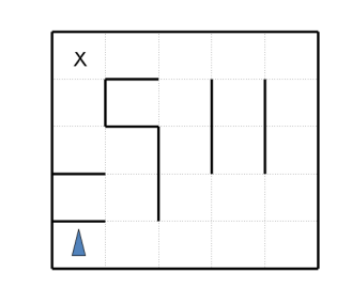
\includegraphics[scale=1]{figures/tp1_maze.png}
\end{center}
At all timesteps, the agent points at direction $d \in$ (N, S, E, W). With a single action, the agent
can either move forward at an adjustable velocity $v$ or turn. The turning actions are left and right, which change
the agent’s direction by 90 degrees. Turning is only permitted when the velocity is zero (and leaves it at zero).
The moving actions are fast and slow. Fast increments the velocity by 1 and slow decrements the velocity by 1;
in both cases the agent then moves a number of squares equal to its \textit{new} adjusted velocity. Any action that
would result in a collision with a wall crashes the agent and is illegal. Any action that would reduce $v$ below 0
or above a maximum speed $V_{max}$ is also illegal. The agent’s goal is to find a plan which parks it (stationary)
on the exit square using as few actions (time steps) as possible.

As an example: if the shown agent is initially stationary, it might first turn to the east using (right), then
move one square east using fast, then two more squares east using fast again. The agent will of course have to
slow to turn.
\begin{itemize}
    \item Quiz:
    \begin{enumerate}
    \item For a grid of size $M \times N$, what is the size of the state space? Assume that all configurations are reachable from the starting state. 
    \begin{solution}
    \\
    $N \times M \times 4 \times (V_{max} + 1)$
    \end{solution}
    \item What is the maximum branching factor of this problem? Assume that illegal actions are simply not returned by the successor function.
    \begin{solution}
    \\
    The maximum branching factor is 3, and this happens when the agent is stationary. While stationary it
    can take the following 3 actions - fast, left, right.
    \end{solution}
    \item Is the Manhattan distance from the agent’s location to the exit’s location admissible?
    \begin{solution}
    \\
    No because it could overestimate the true cost in the case where the average car speed is greater than 1.
    \end{solution}
    \item If we used an inadmissible heuristic in A* tree search, could it change the completeness of the search?
    \begin{solution}\\
    No, A star will still find a final state if there exists a reachable one.
    \end{solution}
    \item If we used an inadmissible heuristic in A* tree search, could it change the optimality of the search?
    \begin{solution}\\
    Yes, we could stop the search whereas there exists a better solution.
    \end{solution}
    \end{enumerate}
    \item Discussion:
    \begin{enumerate}
        \item State and motivate a non-trivial admissible heuristic for this problem.
        \begin{solution}\\
        Some examples of admissible heuristics are:
        \begin{itemize}
            \item The Manhattan distance divided by the speed max.
            \item We can improve the above relaxation by accounting for the deceleration dynamics. In this case the
agent will have to slow down to 0 when it is about to reach the goal. Note that this heuristic will
always return a greater value than the previous one, but is still not an overestimate of the true cost
to reach the goal. We can say that this heuristic dominates the previous one
        \end{itemize}
        \end{solution}
        \item Give a general advantage that an inadmissible heuristic might have over an admissible one.
        \begin{solution}
        \\
        The time to solve an A* tree search problem is a function of two factors: the number of nodes expanded,
and the time spent per node.
An inadmissible heuristic may be faster to compute, leading to a solution that is obtained faster due to
less time spent per node. It can also be a closer estimate to the actual cost function (even though at times
it will overestimate!), thus expanding less nodes.
We lose the guarantee of optimality by using an inadmissible heuristic. But sometimes we may be okay
with finding a suboptimal solution to a search problem.
        \end{solution}
    \end{enumerate}
\end{itemize}
\section*{Exercise 3: Heuristic $\star$}
Consider a search problem where all edges have a unit cost and the optimal solution has cost $C$. Let $h$ be a heuristic which is max\{$h^\star - k$, 0\}, where $h^\star$ is the actual cost to the closest goal and $k$ is a non-negative constant.
\begin{enumerate}
    \item Is $h$ admissible?
    \begin{solution}
    \\
    Yes, indeed $\text{if} \quad h^\star \geq k: h^\star - k \leq h^\star \quad \text{else} \quad 0 \leq h^\star$.
    \end{solution}
    \item Which of the following is the most reasonable description of how much more work will be done (= how many more nodes will be expanded) with heuristic h compared to $h^\star$ , as a function of $k$?
    \begin{enumerate}
        \item Constant in $k$
        \item Linear in $k$
        \item Exponential in $k$
        \item Unbounded
    \end{enumerate}
    \begin{solution}
    %\\
    Exponential in k. At k = 0, only the d nodes on an optimal path to the closest goal are expanded for search depth (= optimal path length) d. At k = max(h), the problem reduces to uninformed search and BFS expands $b \times d$ nodes for branching factor b. In general, all nodes within distance k of the closest goal will have heuristic h = 0 and uninformed search may expand them. Note that search reduces to BFS since A* with h = 0 is UCS and in this search problem all edges have cost 1 so path cost = path length
    \end{solution}
\end{enumerate}
\subsection*{Exercise 4: Search algorithms $\star$}
\begin{center}
    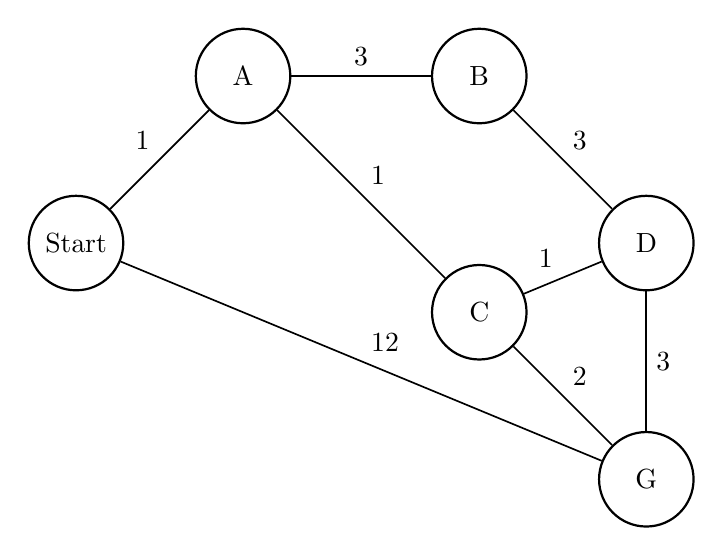
\begin{tikzpicture}[
            -> = stealth, % arrow head style
            %shorten > = 1pt, % don't touch arrow head to node
            auto,
            node distance = 3cm, % distance between nodes
            semithick % line style
        ]

        \tikzstyle{every state}=[
            draw = black,
            thick,
            fill = white,
            minimum size = 12mm
        ]

        \node[state, align=center] (S) {Start};
        \node[state, align=center] (A) [above right of=S] {A};
        \node[state, align=center] (B) [right of=A] {B};
        \node[state, align=center] (C) [below of=B] {C};
        \node[state, align=center] (D) [below right of=B] {D};
        \node[state, align=center] (G) [below of=D] {G};

        \path[-] (S) edge node {1} (A);
        \path[-] (S) edge node {12} (G);
        \path[-] (A) edge node {3} (B);
        \path[-] (A) edge node {1} (C);
        \path[-] (B) edge node {3} (D);
        \path[-] (C) edge node {1} (D);
        \path[-] (C) edge node {2} (G);
        \path[-] (D) edge node {3} (G);

        %\draw[red, dashed] (1, 2) -- (1, -2);
    \end{tikzpicture}
\end{center}

For each of the following search algorithms, give the order in which states are expanded as well as the final path returned by the algorithm. If two nodes are in competition to be expanded, the conflict is resolved by alphabetical order.
\begin{enumerate}
    \item Depth-First search
    \begin{solution}
    \\
    Expansion: S-A-B-D-C-G\\
    Path: S$\rightarrow$A$\rightarrow$B$\rightarrow$D$\rightarrow$C$\rightarrow$G
    \end{solution}
    \item Breadth-First search
    \begin{solution}
    \\
    Expansion: S-A-G\\
    Path: S$\rightarrow$G
    \end{solution}
    \item Uniform-Cost search
    \begin{solution}
    \\
    Expansion: S-A-C-D-B-G\\
    Path: S$\rightarrow$A$\rightarrow$C$\rightarrow$G
    \end{solution}
    \item Consider the following heuristics:
    \begin{table}[h]
        \centering
        \begin{tabular}{|c|c|c|}
        \hline
            State & $h_1$ & $h_2$ \\ \hline
            S & 5 & 4\\ \hline
            A & 3 & 2\\ \hline
            B & 6 & 6\\ \hline
            C & 2 & 1\\ \hline
            D & 3 & 3\\ \hline
            G & 0 & 0\\ \hline
        \end{tabular}
        \caption{2 possible heuristics}
        \label{tab:my_label}
    \end{table}
    which one is not admissible? Why?
    \begin{solution}
    \\
    h1 is not admissible because the real cost from S to G is 4 which is smaller than 5.
    \end{solution}
    \item Use the admissible heuristic to apply A* algorithm.
    \begin{solution}
    \\
    Expansion: S-A-C-G
    Path: S$\rightarrow$A$\rightarrow$C$\rightarrow$G
    \end{solution}
\end{enumerate}
\subsection*{Exercise 5: The hive $\star$}
The hive of insects needs your help. You control an insect in a rectangular maze-like environment
of size $M \times N$, as shown on the Figure below. At each time-step,
the insect can move into a free adjacent cell or stay in its current
location. All actions have a unit cost. \\
In this particular case, the insect must pass through a series of partially
flooded tunnels, as illustrated by the grey cells on the map. The insect can hold its breath for $A$ time-steps in a row. Moving
into a flooded cell requires your insect to consume 1 unit of air, while
moving into a free cell refills its air supply.
\begin{figure}[H]
    \centering
    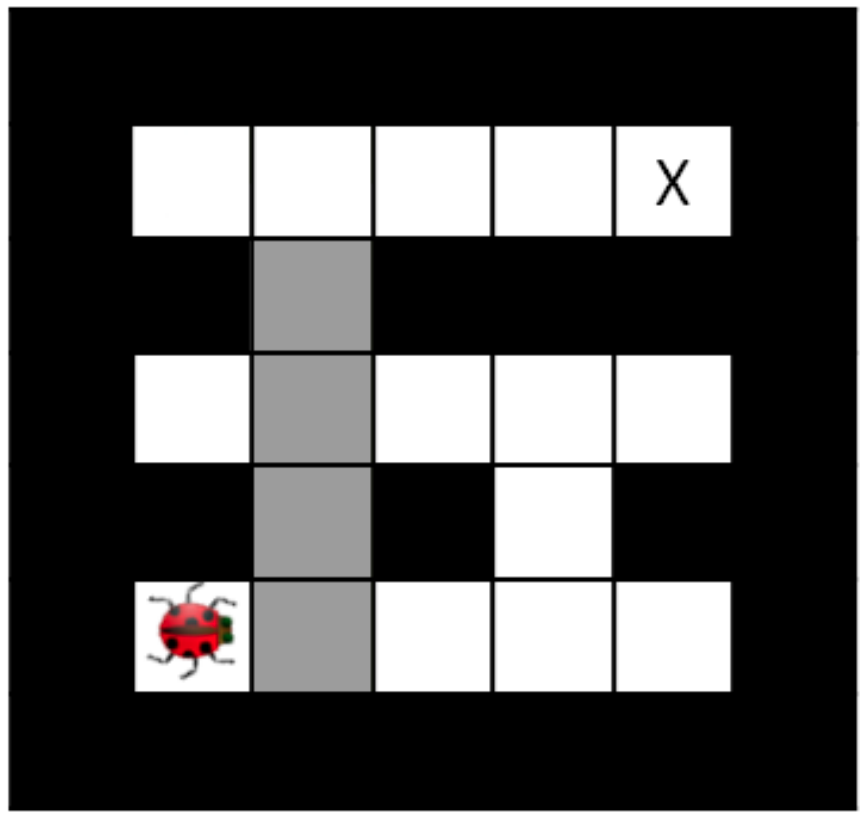
\includegraphics[width=.2 \textwidth]{figures/hive.png}
    \label{fig:hive}
\end{figure}
\begin{itemize}
    \item Give a minimal state space for this problem (i.e., do not include extra information). You should
answer for a general instance of the problem, not the specific map above.
\begin{solution}
\\
The position of the insect  as well as the number of unit of air it has left. $s = (x, y, u_a) \in \{1, \hdots, M\} \times \{1, \hdots N\} \times \{1, \hdots, A\}$.
\end{solution}
    \item Give the size of your state space.
    \begin{solution}
    \\
    $M\times N \times A$ 
    \end{solution}
\end{itemize}
   \section*{Supplementary materials}
   \href{http://ai.berkeley.edu/sections/section_0_v55LOfoUUwiW1k6Nchnk3Dw6WQuTW8.pdf}{Berkeley 1}\\
   \href{http://ai.berkeley.edu/sections/section_1_0hzy6TFupb1Z3bckfRXdC5KYpsdZOE.pdf}{Berkeley 2}\\
   Chapter 3 of reference book.
\end{document}
